\chapter[Measuring FD PMT Gain Variance with CalA Data]{\centering Measuring Fluorescence Detector Photomultiplier Gain Variance with CalA Data \\}\label{Ch:GainVariance}

Measuring Gain Variance of FD PMT with CalA Data
\begin{itemize}
\item Measuring Gain Variance in the lab did not work. Equipment was not sensitive enough to the low current.
\item There was issues with calibrating the LED light source with another PMT (QE curve and wavelength response not the same?)
\item Using Low/Standard measurements of CalA to find Gain Variance Ratio
\item Two different methods
\item Bootstrap method to find uncertainties on Method 2
\end{itemize}

\section{Motivation}
\
- Background

- Why?

The absolute value of the gain variance cannot be found but using the CalA data a relative change can be found. This is useful for the collaboration simulations as a Gain variance is coded for the PMT at standard voltage settings. Finding out the relative change in gain variance would be useful to be used for simulations of the FD PMTs at a lower voltage settings (eg. 600V).

\section{Using CalA to measure relative changes in Gain Variance}

I am using CalA data from the FD telescopes to measure the relative changes in PMT gain variance as the gain was changed by a factor of 10. CalA data is calibration data used to monitor any changes in PMT gain as a function of time. CalA is performed at the beginning and end of a nightly observation while FDs are operated. Pulses of light are piped via fibre optics cables which is pointed at each of the Fd telescope cameras. Each CalA run is a set of 50 pulses which have a width of approximately 60 $\mu$s.

\textbf{show image of CalA pulse}

One of the values that can be calculated from the CalA is denoted K$_{\mathrm{V}}$. The value K$_{\mathrm{V}}$ is calculated via:
\begin{equation}
\mathrm{K}_{\mathrm{V}} = \frac{\mathrm{Mean}}{\mathrm{Sigma}^2} = \frac{10}{2 \times \mathrm{G} (1 + \mathrm{V}_{\mathrm{G}}) \times \mathrm{F}}
\end{equation}
The Mean is the average ADC count of the observed CalA pulse seen in the FD pixel. The Sigma$^2$ is the variance calculated around a fit to the signal in ADC$^2$. The signal has a slope due to the effects of a capacitor used to remove the DC component of the signal. The slope is proportional to the time constant of the capacitor employed. G is the PMT gain, F is the noise equivalent bandwidth (Hz) and V$_{\mathrm{G}}$ is the PMT gain variance.


The method used to measure the ratio in gain variance is to take the calculated means and sigmas from the pulses and then finding a ratio between the K$_{\mathrm{V}}$ and Gains at the two different voltage settings.
\begin{eqnarray}
\mathrm{K} = \frac{\mathrm{Mean}}{\mathrm{Sigma}^2} &=& \frac{10}{2 \times \mathrm{G} (1 + \mathrm{V}_{\mathrm{G}}) \times \mathrm{F}} \\ 
\frac{\left(\mathrm{K}_{\mathrm{V}}\right)_{\mathrm{Low}}}{\left(\mathrm{K}_{\mathrm{V}}\right)_{\mathrm{Stand}}} &=& \frac{\mathrm{Mean}_{\mathrm{Low}}}{\mathrm{Sigma}^2_{\mathrm{Low}}} \div \frac{\mathrm{Mean}_{\mathrm{Stand}}}{\mathrm{Sigma}^2_{\mathrm{Stand}}} \\ 
\frac{\mathrm{Mean}_{\mathrm{Low}}}{\mathrm{Sigma}^2_{\mathrm{Low}}} \div \frac{\mathrm{Mean}_{\mathrm{Stand}}}{\mathrm{Sigma}^2_{\mathrm{Stand}}} &=& \frac{\mathrm{G}_{\mathrm{Stand}} (1 + \mathrm{V}_{\mathrm{G}})_{\mathrm{Stand}}}{\mathrm{G}_{\mathrm{Low}} (1 + \mathrm{V}_{\mathrm{G}})_{\mathrm{Low}}} \\
\frac{\mathrm{G}_{\mathrm{Stand}}}{\mathrm{G}_{\mathrm{Low}}} &=& \frac{\mathrm{Mean}_{\mathrm{Stand}}}{\mathrm{Mean}_{\mathrm{Low}}} \\
\frac{(1 + \mathrm{V}_{\mathrm{G}})_{\mathrm{Low}}}{(1 + \mathrm{V}_{\mathrm{G}})_{\mathrm{Stand}}} &=& \frac{\mathrm{Sigma}^2_{\mathrm{Low}} \times \mathrm{Mean}^2_{\mathrm{Stand}}}{\mathrm{Sigma}^2_{\mathrm{Stand}} \times \mathrm{Mean}^2_{\mathrm{Low}}}
\end{eqnarray}

\section{Electronic Noise}

I investigated the consistency of the electronic noise across a set of 50 CalA traces. The consistency was looked at as there is only about 140 bins of noise before each of the signal pulse starts. Therefore finding an accurate mean and variance of the electronic noise on individual pulses is difficult. An accurate measurement of the electronic noise mean and variance was required as the measured gain variance ratio was only a few percent.

\textbf{Need to show electronic noise as function of time.}

An example of a pixel electronic noise trace is shown in Fig. \ref{}. It can be seen in this figure that stitching all of the noise bins from the 50 traces is remarkably stable. This result allows for all the noise for a single PMT pixel to be place into a histogram to find a more accurate value for the mean and variance.

\begin{figure} % Electronic Noise Distribution
\centering
\begin{subfigure}[b]{0.95\textwidth}
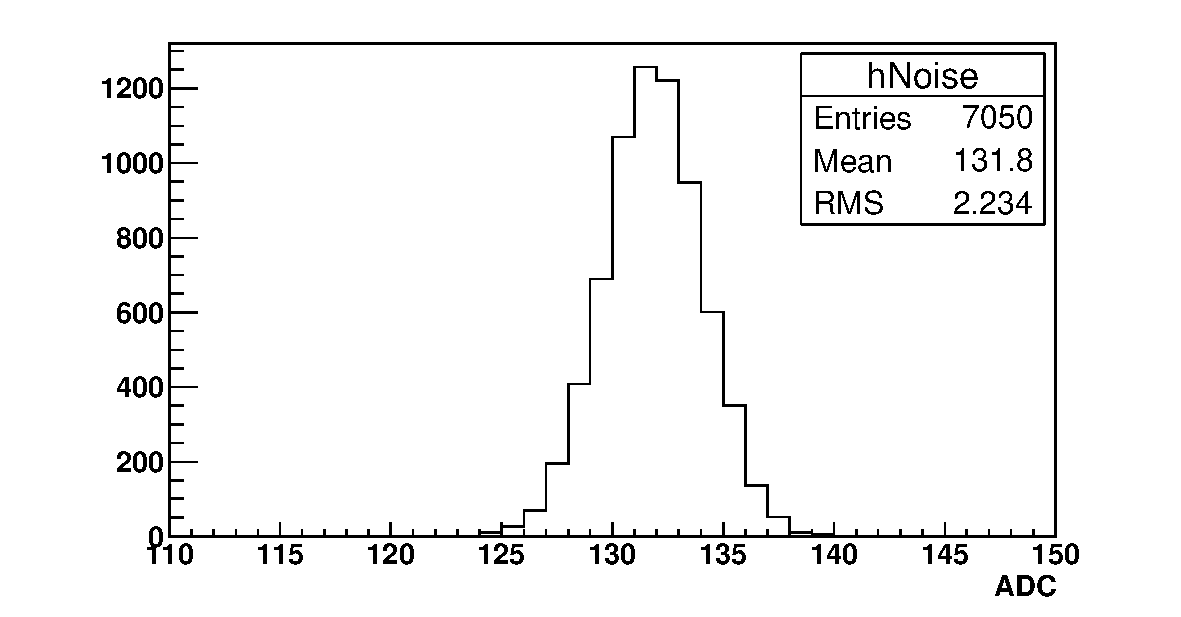
\includegraphics[width=\textwidth]{chapters/graphs/GainVarsMeas/LL_m04_2016-06-11/example_NoiseHist1.pdf}
\caption{Standard HV}
\end{subfigure}
\vspace{3mm}
\begin{subfigure}[b]{0.95\textwidth}
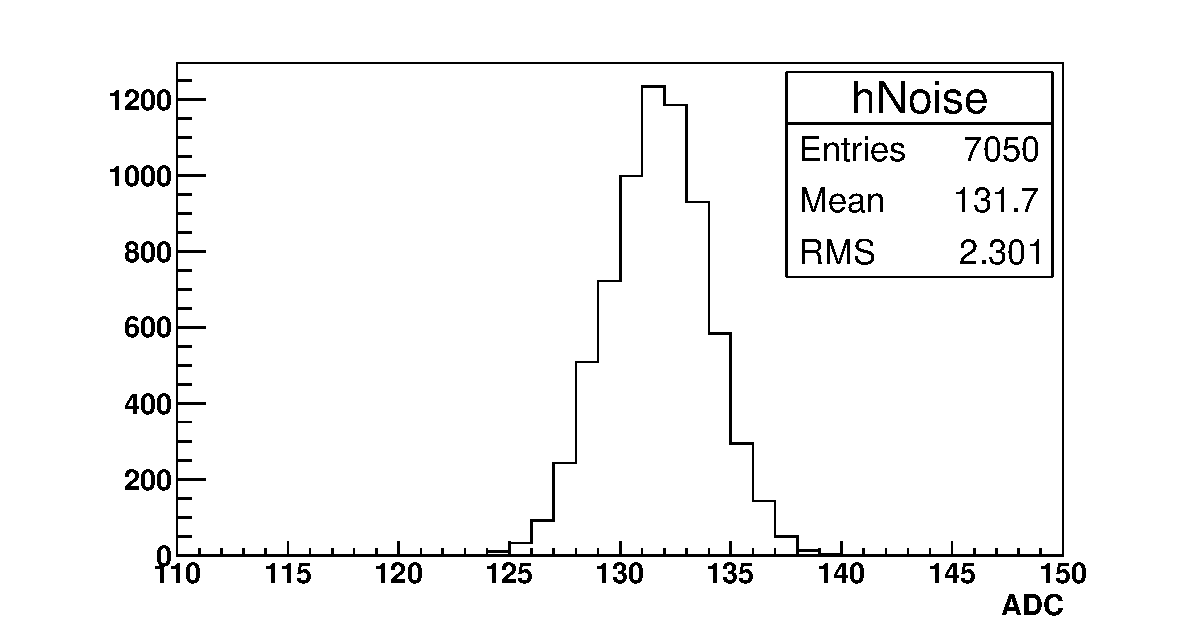
\includegraphics[width=\textwidth]{chapters/graphs/GainVarsMeas/LL_m04_2016-06-11/example_NoiseHist2.pdf}
\caption{Lower HV}
\end{subfigure}
\caption{Sample of the observed electronic noise observed for a single pixel within Los Leones telescope 4. Electronic noise outside of the PMT so will be the same separate from the HV setting across the PMT.}
\end{figure}

\section{Pairs Method}

For both standard and reduced voltage settings 50 sets of pulses are recorded for the CalA analysis. The pair method involves taking single CalA shots from standard and lower voltage settings and fitting an exponential to the signal. The fitted exponential is used to find the mean value at the top of the signal and the variance around the fit. For each pixel 50 values for the Gain Variance ratio is found and this is repeated for the 440 pixels within the FD telescope.

Fig. \ref{fig:CalAMeanADC_Pairs} shows the average ADC count found across a camera for a FD telescope. The pattern follow how the camera is illuminated by the LED pointing at the camera. It shows that the spot is brightness in the middle and the intensity drops off towards the edges \textbf{need to add in diagram of labelled pixel no. across a FD camera}. There are uncertainties on the averages but are smaller then the displayed points. The variance measured in Fig. \ref{fig:CalAVarsADC_Pairs} shows an expected pattern too. The variance is proportional to the mean and is expected to follow a similar shape. This will not be exact but a good indicator of whether the variance was calculated correctly.

\begin{figure} % Mean Plot
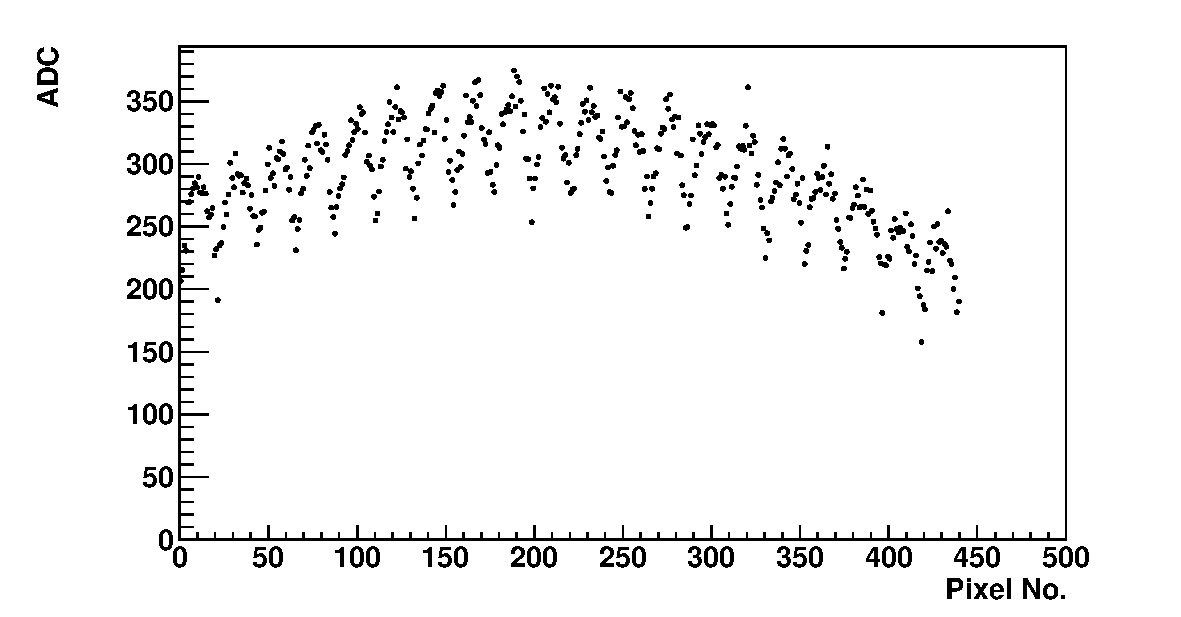
\includegraphics[width=\textwidth]{chapters/graphs/GainVarsMeas/LL_m04_2016-06-11/Set0and2/meanHist_StandHV_Pairs_set0and2.pdf}
\caption{Mean measured at Standard HV for Los Leones Mirror 4. CalA data taken on the 11-06-2016.}
\vspace{3mm}
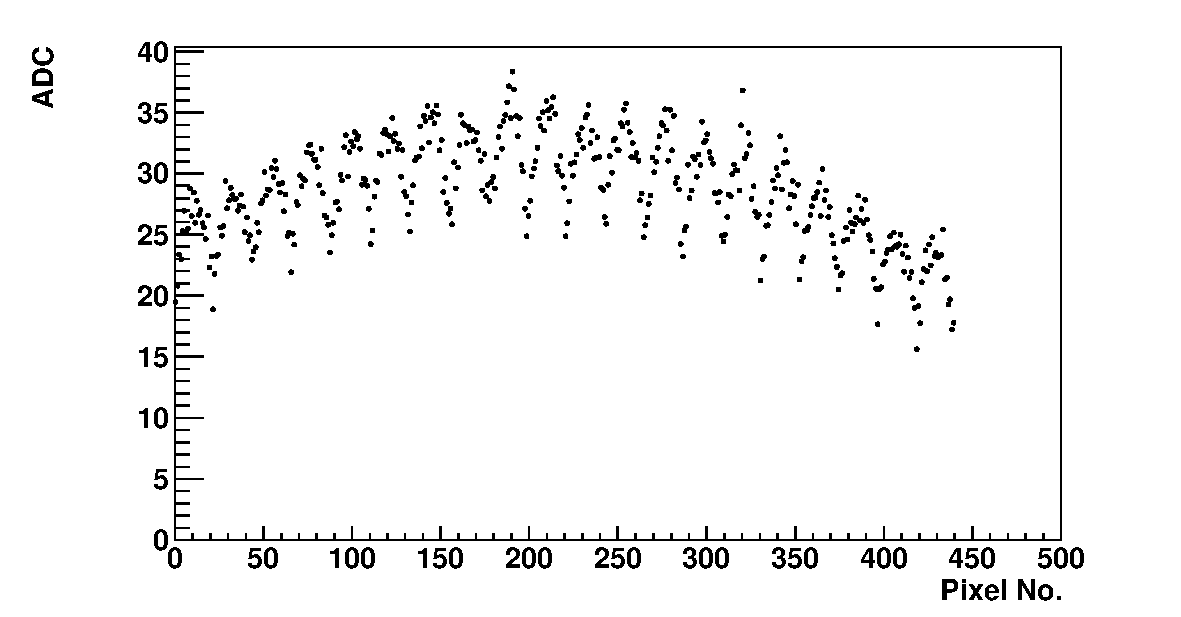
\includegraphics[width=\textwidth]{chapters/graphs/GainVarsMeas/LL_m04_2016-06-11/Set0and2/meanHist_LowHV_Pairs_set0and2.pdf}
\caption{Mean measured at Lower HV for Los Leones Mirror 4. CalA data taken on the 11-06-2016.} \label{fig:CalAMeanADC_Pairs}
\end{figure}

\begin{figure} % Variance Plot
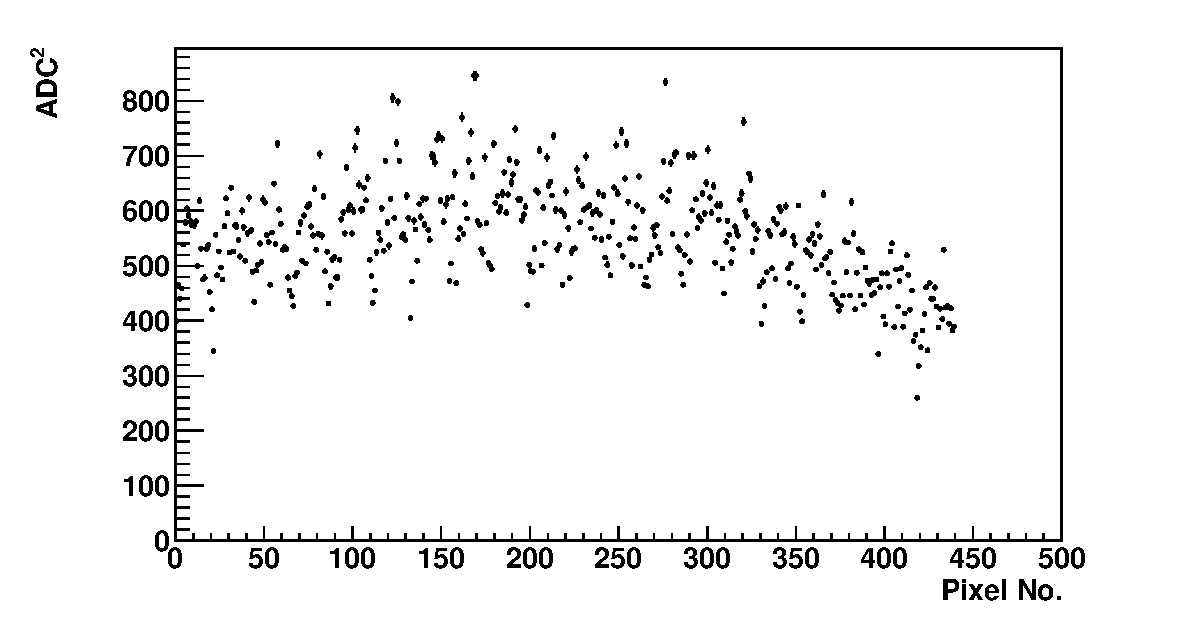
\includegraphics[width=\textwidth]{chapters/graphs/GainVarsMeas/LL_m04_2016-06-11/Set0and2/varianceHist_StandHV_Pairs_set0and2.pdf}
\caption{Variance measured at Standard HV for Los Leones Mirror 4. CalA data taken on the 11-06-2016.}
\vspace{3mm}
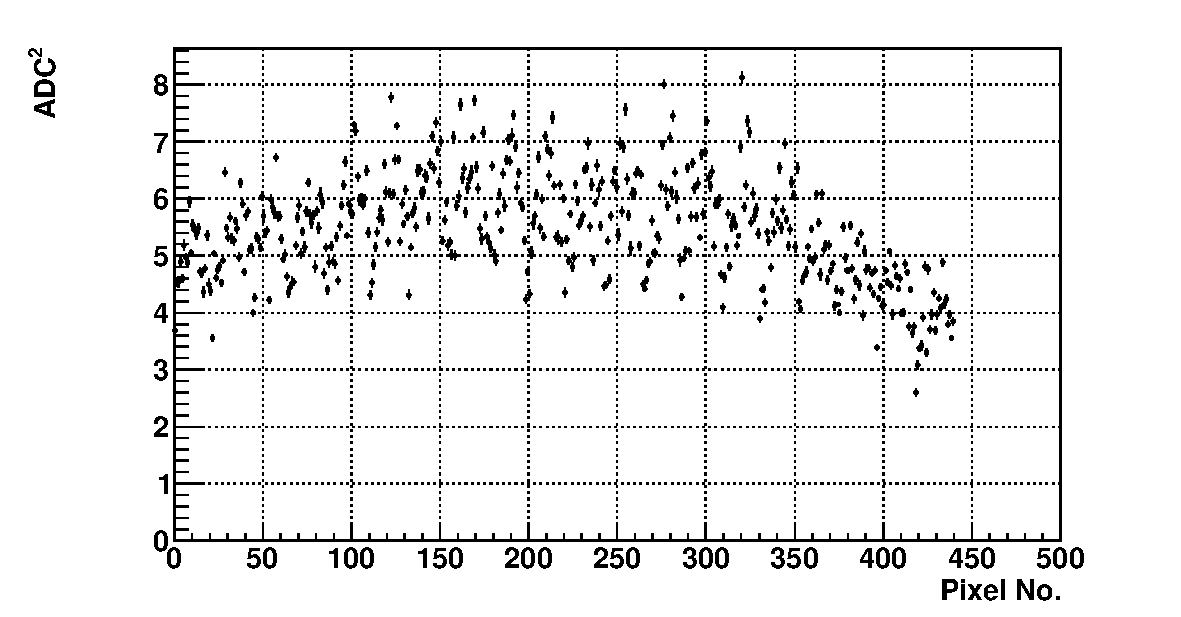
\includegraphics[width=\textwidth]{chapters/graphs/GainVarsMeas/LL_m04_2016-06-11/Set0and2/varianceHist_LowHV_Pairs_set0and2.pdf}
\caption{Varaince measured at Lower HV for Los Leones Mirror 4. CalA data taken on the 11-06-2016.} \label{fig:CalAVarsADC_Pairs}
\end{figure}

\subsection{Results}

Fig. \ref{fig:GainVarsRatio_Hist_PairsEx} and Fig. \ref{fig:GainVarsRatioVsPixel_PairsEx} shows a demonstration of using the Pairs Method to calculate the Gain Variance Ratio. The CalA data used was taken on the night of the 11-06-2016 by Los Leones Mirror 4. The mean value in Fig. \ref{fig:GainVarsRatio_Hist_PairsEx} shows a 3.7\% change in the ratio which translate to a 10\% change in the actual value of the PMT gain variance.

Fig. \ref{fig:GainVarsRatioVsPixel_PairsEx} shows the gain variance ratio measured per pixel. There can be seen no major structure or pattern. This is desired as the Gain variance is tired to individual PMTs and it would not be a great sign if the ratio followed a pattern like what was seen for the means and variances.

\begin{figure} % Gain Variance Plot
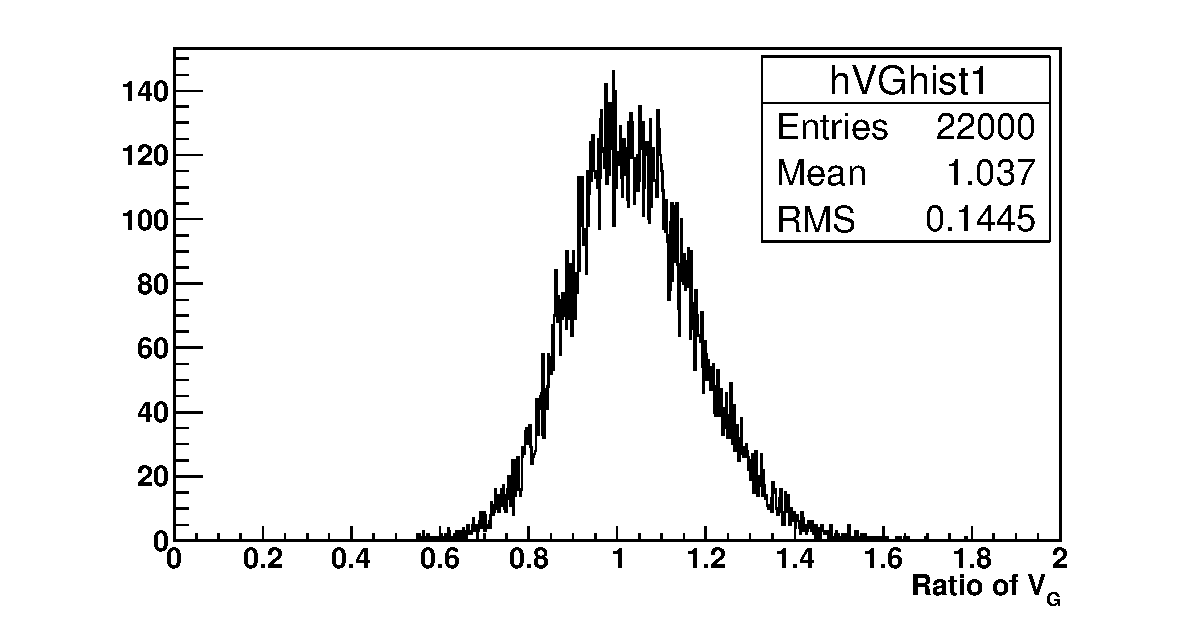
\includegraphics[width=\textwidth]{chapters/graphs/GainVarsMeas/LL_m04_2016-06-11/Set0and2/GainVairanceHist_Pairs.pdf}
\caption{Histogram of the all the pairs methods for Los Leones Mirror 4. CalA data was taken on the 11/06/2016 at both Standard and Lower gain settings. There are 50 traces for each of the 440 pixels recorded at both gain settings. } \label{fig:GainVarsRatio_Hist_PairsEx}
\vspace{3mm}
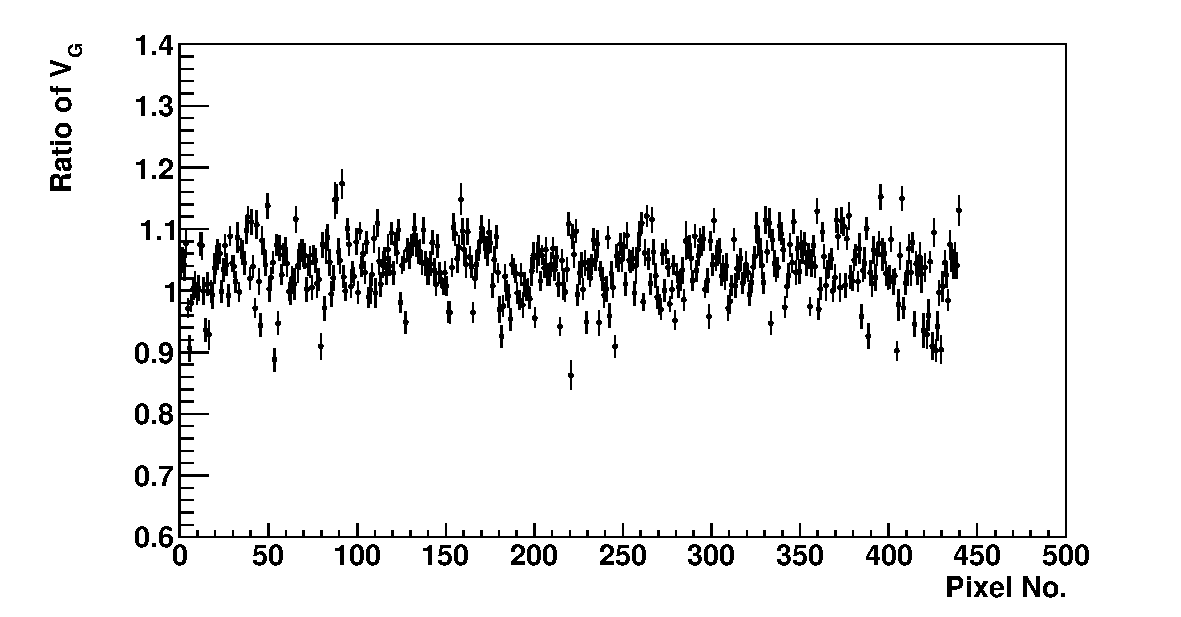
\includegraphics[width=\textwidth]{chapters/graphs/GainVarsMeas/LL_m04_2016-06-11/Set0and2/GainVars_Vs_Pixel_GainVariance_Pairs_Set0and2.pdf}
\caption{} \label{fig:GainVarsRatioVsPixel_PairsEx}
\end{figure}

\section{Averaging Sets of Traces Method}

Instead of calculating the Gain Variance ratio on pairs of CalA traces then finding an average value the 50 traces for each set are stacked. This forms an average trace consisting of the 50 traces. To find the mean and variances of the noise a linear line of form f(x) = x is fitted to the first 140 bins. the fitted x is used as the mean and the variance is calculated around this value. Next an exponential is fitted to the signal. The value of the fit at the top of the signal is used as the mean while the variance is calculated around the fitted exponential.  

\begin{figure} % Mean Plot
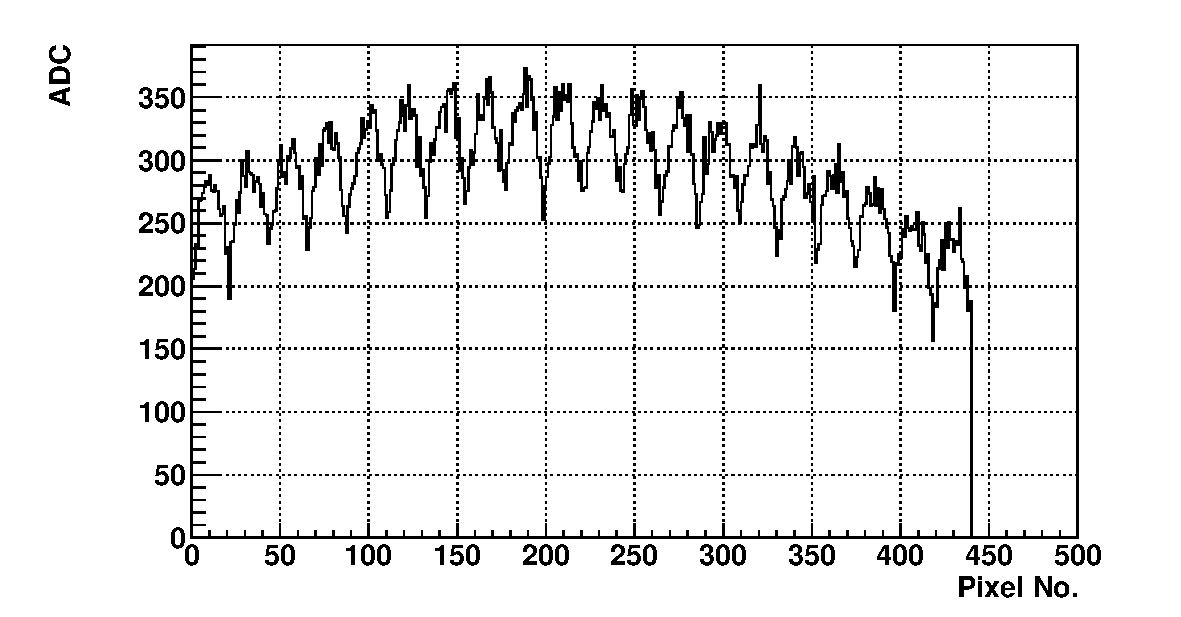
\includegraphics[width=\textwidth]{chapters/graphs/GainVarsMeas/LL_m04_2016-06-11/Set0and2/meanHist_StandHV_Average_set0and2.pdf}
\caption{}\label{fig:MeanVsPixel_StandardHV_Average}
\vspace{3mm}
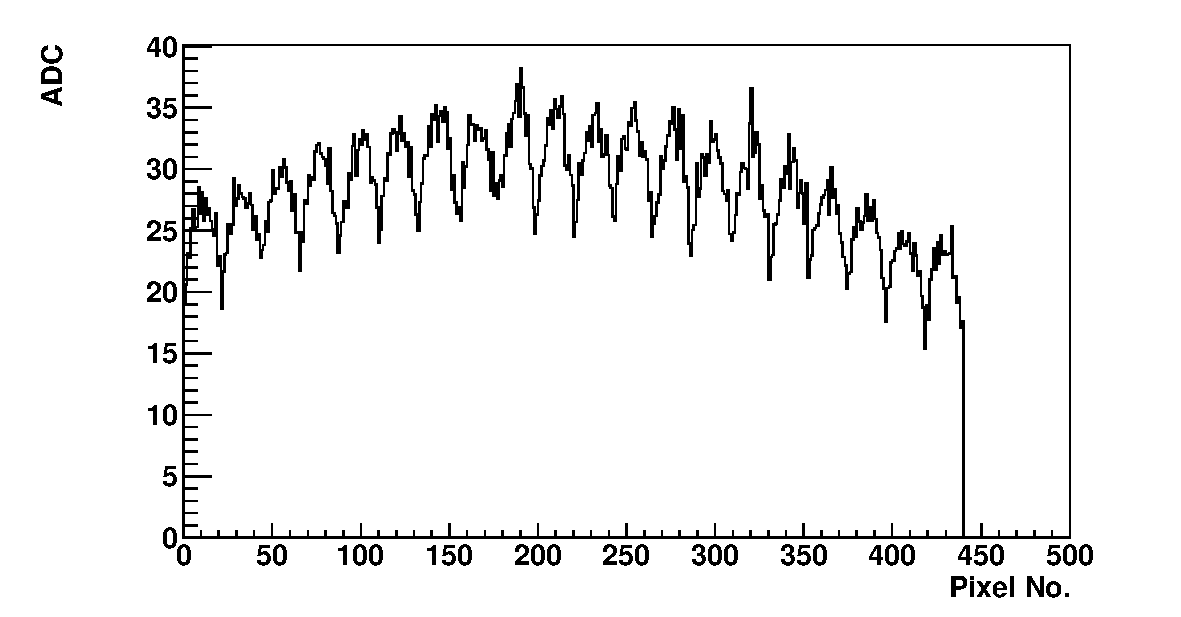
\includegraphics[width=\textwidth]{chapters/graphs/GainVarsMeas/LL_m04_2016-06-11/Set0and2/meanHist_LowHV_Average_set0and2.pdf}
\caption{}\label{fig:MeanVsPixel_LowerHV_Average}
\end{figure}

\begin{figure} % Variance Plot
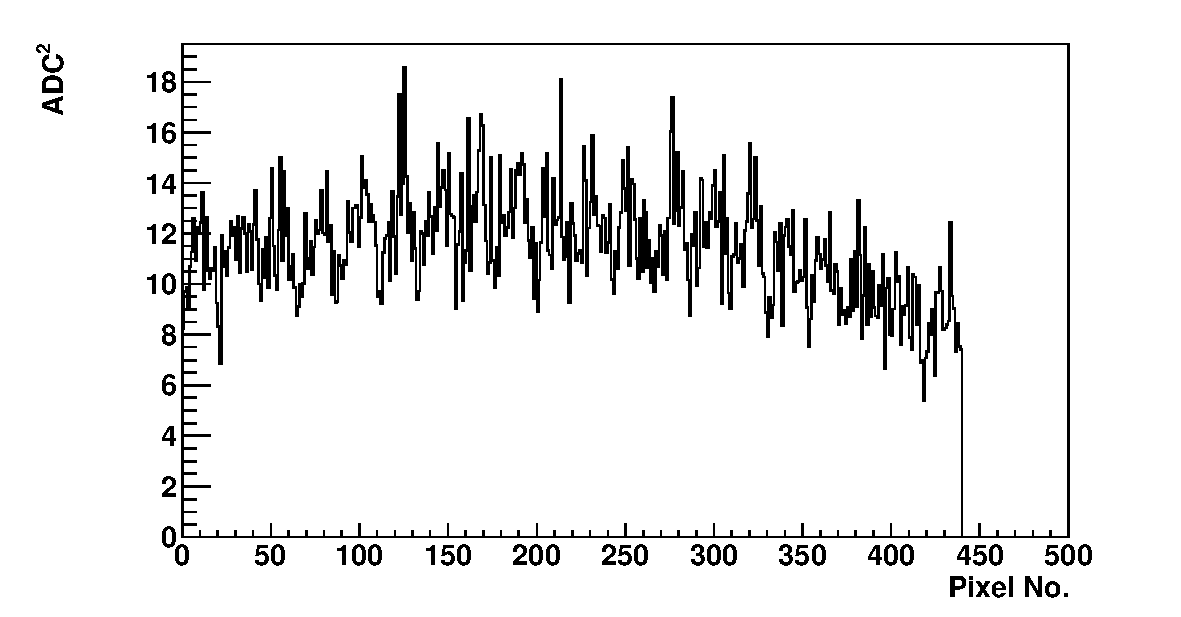
\includegraphics[width=\textwidth]{chapters/graphs/GainVarsMeas/LL_m04_2016-06-11/Set0and2/varianceHist_StandHV_Average_set0and2.pdf}
\caption{}\label{fig:VarsVsPixel_StandardHV_Average}
\vspace{3mm}
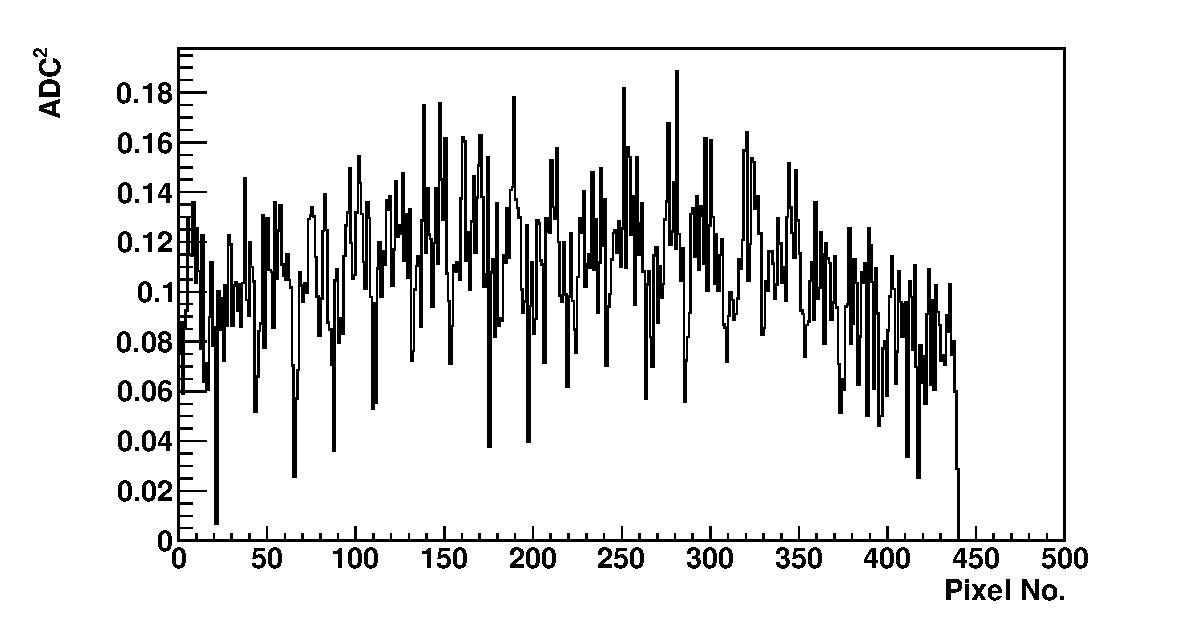
\includegraphics[width=\textwidth]{chapters/graphs/GainVarsMeas/LL_m04_2016-06-11/Set0and2/varianceHist_LowHV_Average_set0and2.pdf}
\caption{}\label{fig:VarsVsPixel_LowerHV_Average}
\end{figure}

\subsection{Results}

There is a larger spread in the histogram of calculated Gain Variance ratio then when the Pairs Method was employed. One good property is that no visible structure or pattern can be seen. There are definitely some extreme values of the ratio measured. To see what could cause the large outliers I had a look at the reduced chi-square of the fitted function to the noise and signal. There was no obvious problems when the looking at the chi-squares as a function of pixel number for the signal. Examples are shown in Fig. \ref{fig:Chi2VsPixel_Signal_StandHV_Average} and Fig. \ref{fig:Chi2VsPixel_Signal_LowerHV_Average}. Examining the reduced chi-square of the fits to the noise it was seen that there was some large values. This was shown in Fig. \ref{fig:Chi2VsPixel_Noise_StandHV_Average} and Fig. \ref{fig:Chi2VsPixel_Noise_LowerHV_Average}. What was causing these weird fits was one or more of the noise bins having a larger deviation then expected from the measured average. \textbf{Add in plot showing off this behaviour}. This led to the process of investigating whether Least Trimmed Squares would be useful.

\begin{figure} % Gain Variance Plot
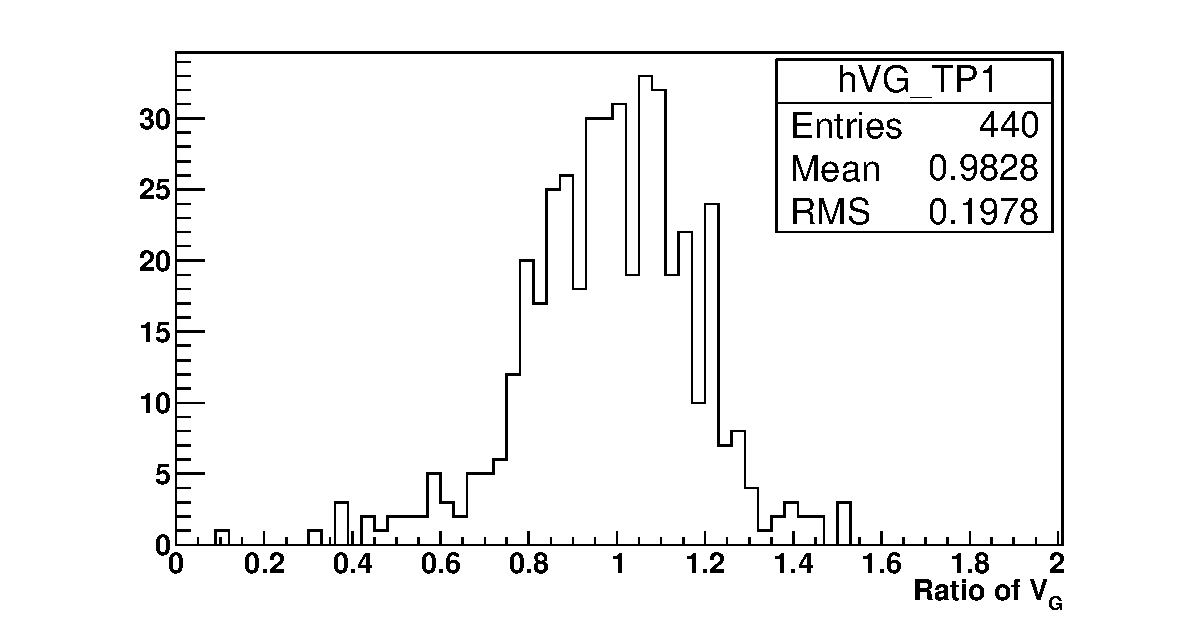
\includegraphics[width=\textwidth]{chapters/graphs/GainVarsMeas/LL_m04_2016-06-11/Set0and2/GainVairanceHist_Average_Method1.pdf}
\caption{}\label{fig:GainVarsRatioHist_Average}
\vspace{3mm}
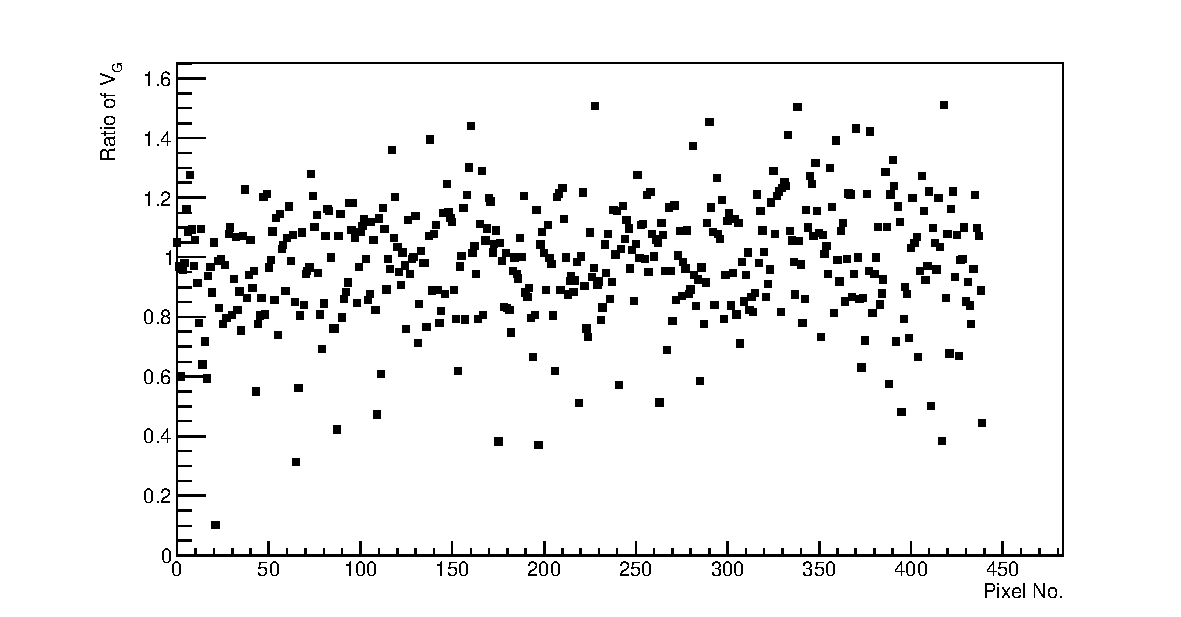
\includegraphics[width=\textwidth]{chapters/graphs/GainVarsMeas/LL_m04_2016-06-11/Set0and2/GainVars_Vs_Pixel_GainVariance_Average_Method1_Set0and2.pdf}
\caption{}\label{fig:GainsVarsRatioVsPixel_Average}
\end{figure}

\begin{figure}% Signal Chi2
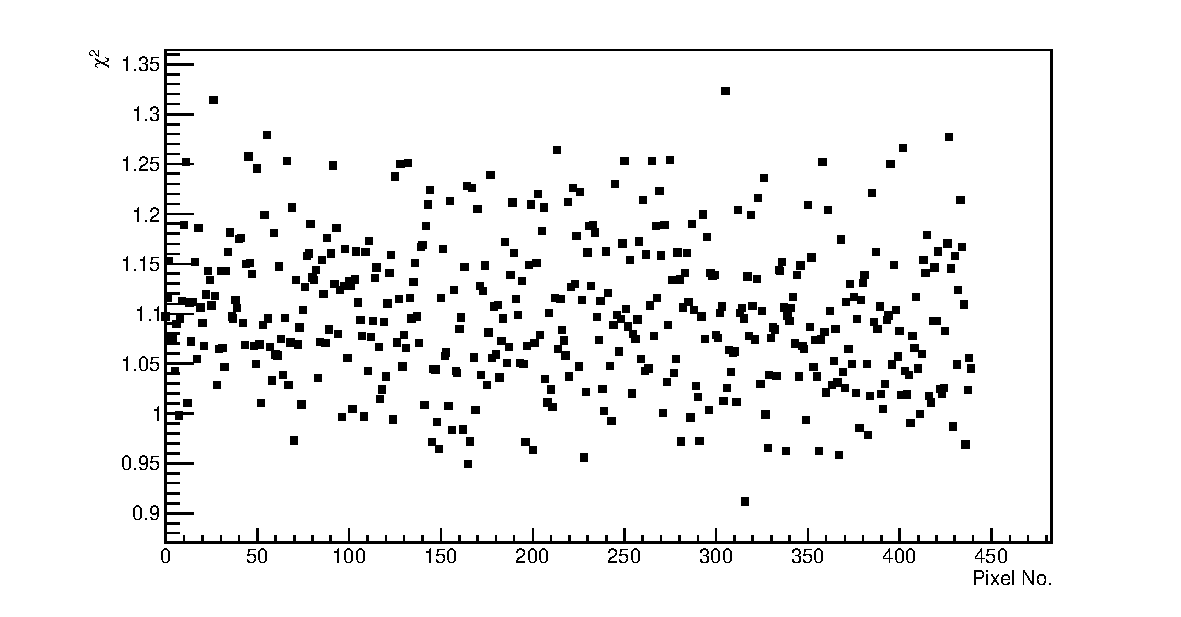
\includegraphics[width=\textwidth]{chapters/graphs/GainVarsMeas/LL_m04_2016-06-11/Set0and2/Chi2_AverageMethod_Signal_StandHV.pdf}
\caption{Reduced Chi-square for fitted exponential on the signal for CalA events measured at Standard HV.}\label{fig:Chi2VsPixel_Signal_StandHV_Average}
\vspace{3mm}
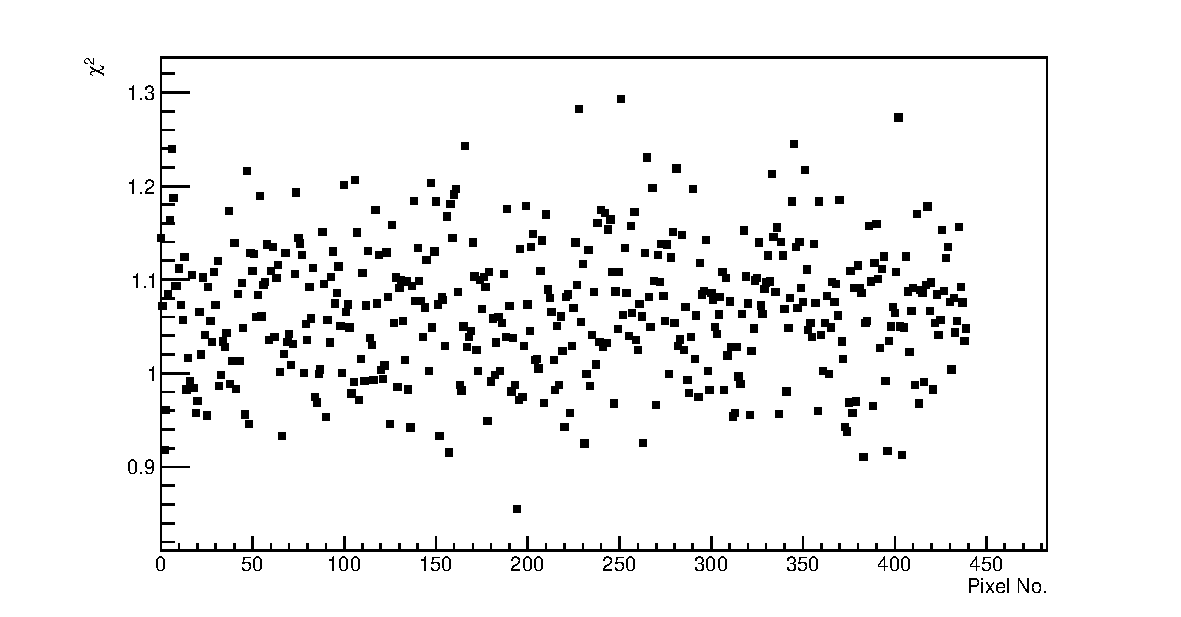
\includegraphics[width=\textwidth]{chapters/graphs/GainVarsMeas/LL_m04_2016-06-11/Set0and2/Chi2_AverageMethod_Signal_LowHV.pdf}
\caption{Reduced Chi-square for fitted exponential on the signal for CalA events measured at Lower HV.}\label{fig:Chi2VsPixel_Signal_LowerHV_Average}
\end{figure}

\begin{figure}% Noise Chi2
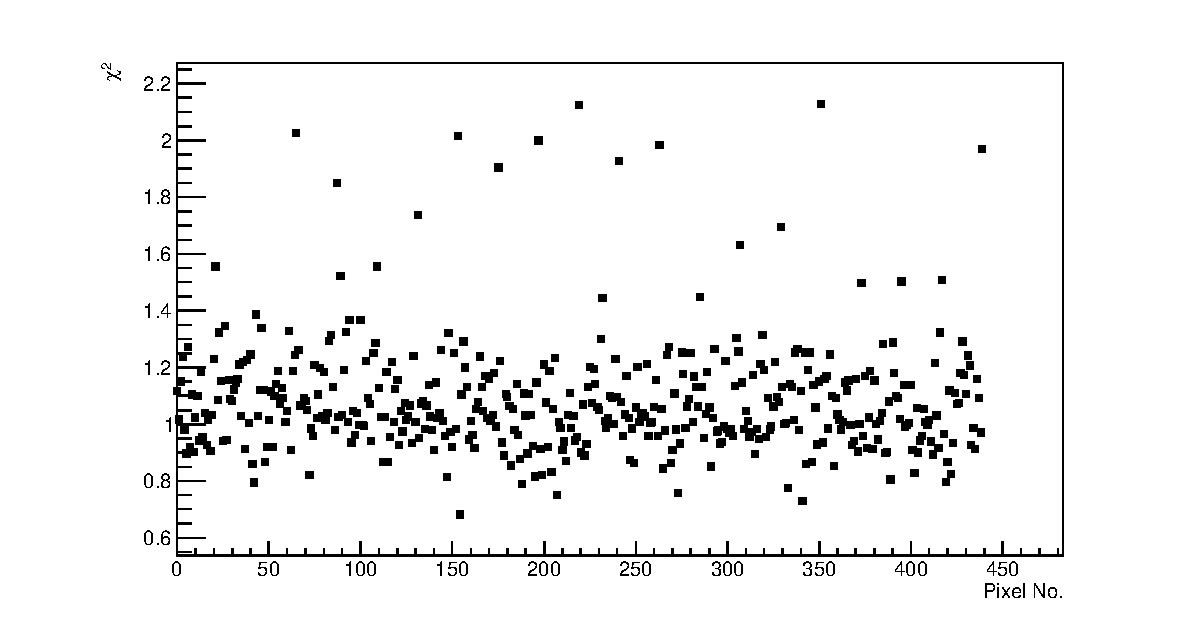
\includegraphics[width=\textwidth]{chapters/graphs/GainVarsMeas/LL_m04_2016-06-11/Set0and2/Chi2_AverageMethod_Noise_StandHV.pdf}
\caption{Reduced Chi-square for fitted line on the signal for CalA events measured at Standard HV.}\label{fig:Chi2VsPixel_Noise_StandHV_Average}
\vspace{3mm}
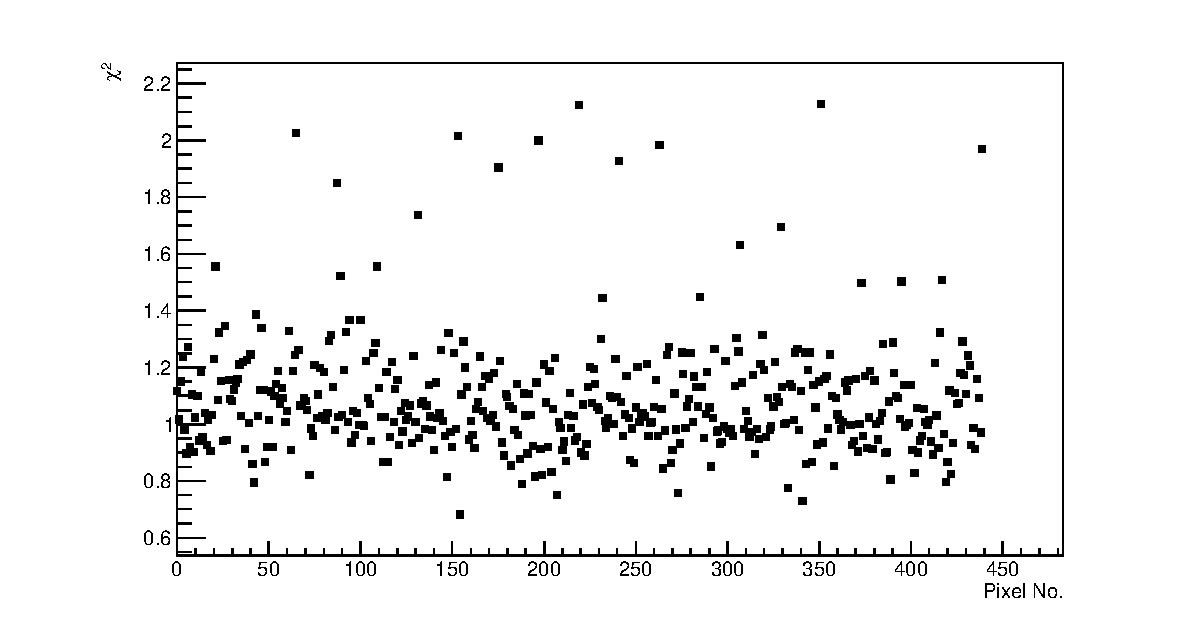
\includegraphics[width=\textwidth]{chapters/graphs/GainVarsMeas/LL_m04_2016-06-11/Set0and2/Chi2_AverageMethod_Noise_LowHV.pdf}
\caption{Reduced Chi-square for fitted line on the signal for CalA events measured at Lower HV.}\label{fig:Chi2VsPixel_Noise_LowerHV_Average}
\end{figure}

\section{Result of Averaging Sets of Traces Method with Least Trimmed Squares}

Least Trimmed Square is the method that involves removing points that have the greatest sigma away from an initial fit. A point is removed one at a time with the fit repeated and the reduced chi-square checked. This method is repeated until the reduced chi-square is below a threshold.


\begin{figure} % Gain Variance Plot
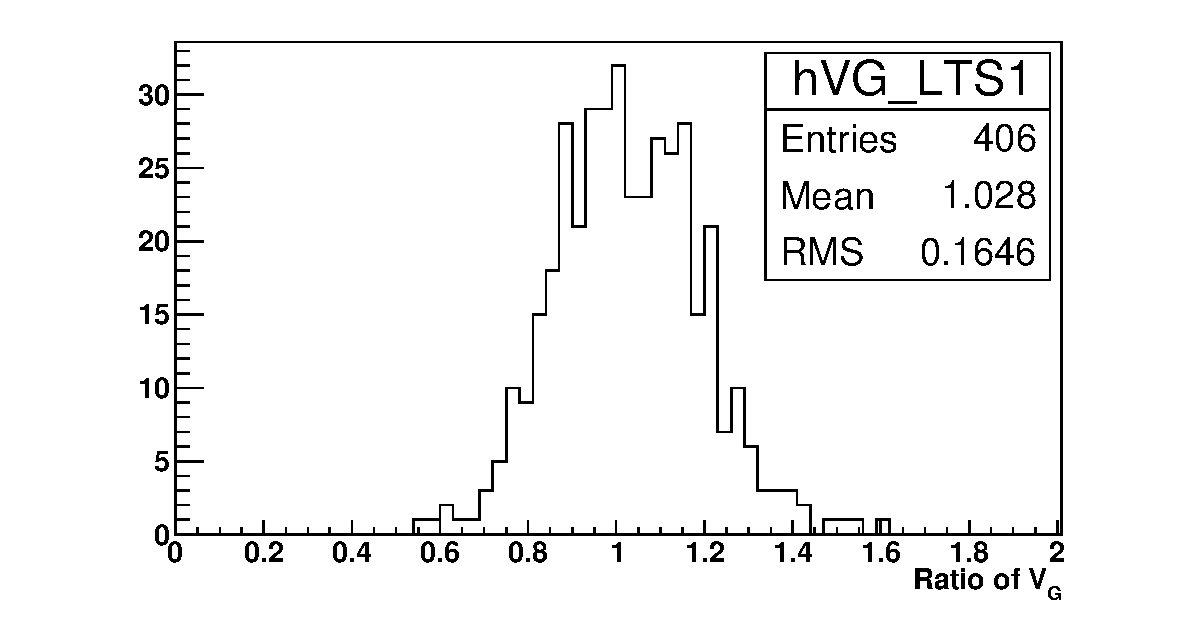
\includegraphics[width=\textwidth]{chapters/graphs/GainVarsMeas/LL_m04_2016-06-11/Set0and2/GainVairanceHist_Average_LTS.pdf}
\caption{}
\vspace{3mm}
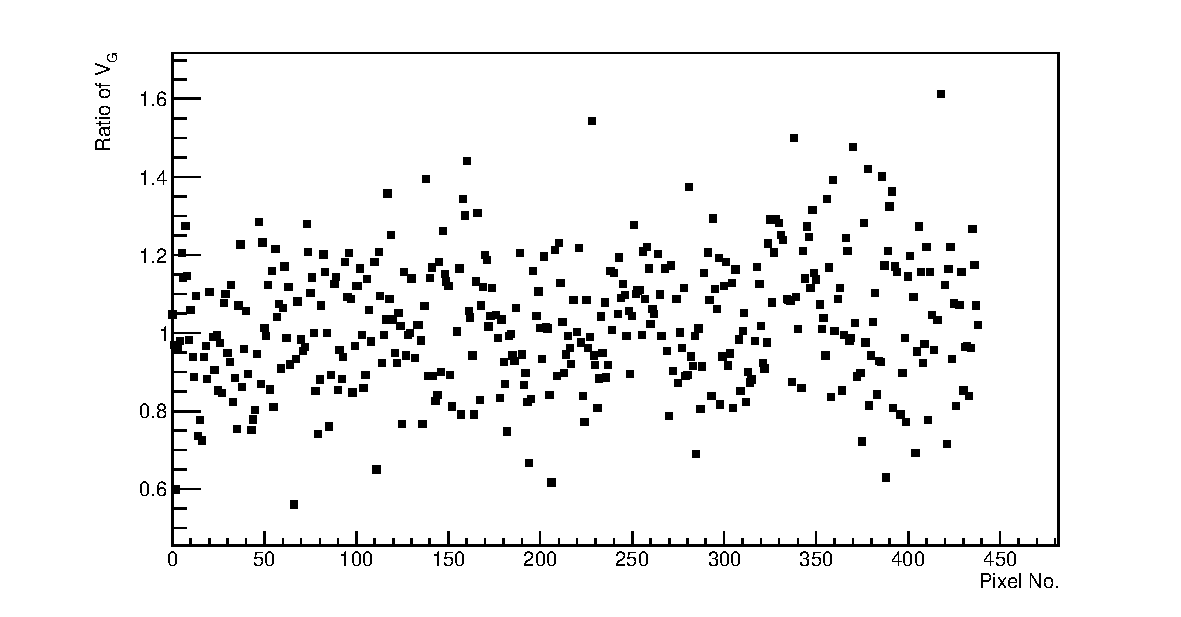
\includegraphics[width=\textwidth]{chapters/graphs/GainVarsMeas/LL_m04_2016-06-11/Set0and2/GainVars_Vs_Pixel_GainVariance_AverageLTS_Set0and2.pdf}
\caption{}
\end{figure}

\section{Result of Averaging Sets of Traces Method using Noise Distribution}

\begin{figure} % Gain Variance Plot
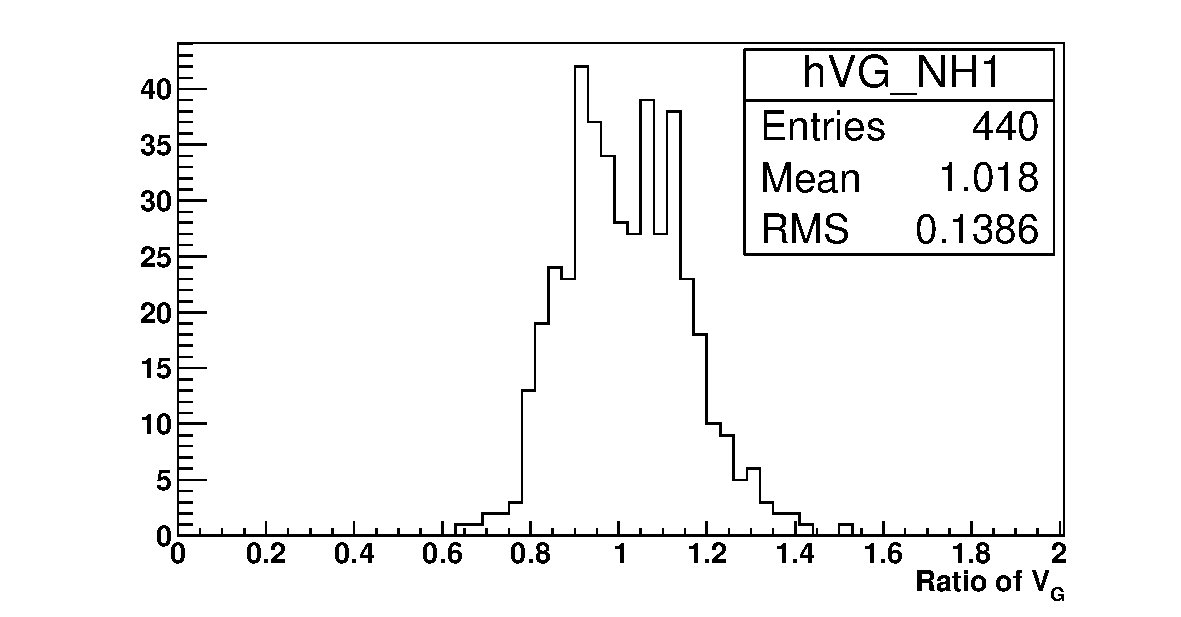
\includegraphics[width=\textwidth]{chapters/graphs/GainVarsMeas/LL_m04_2016-06-11/Set0and2/GainVairanceHist_Average_Method2.pdf}
\caption{}
\vspace{3mm}
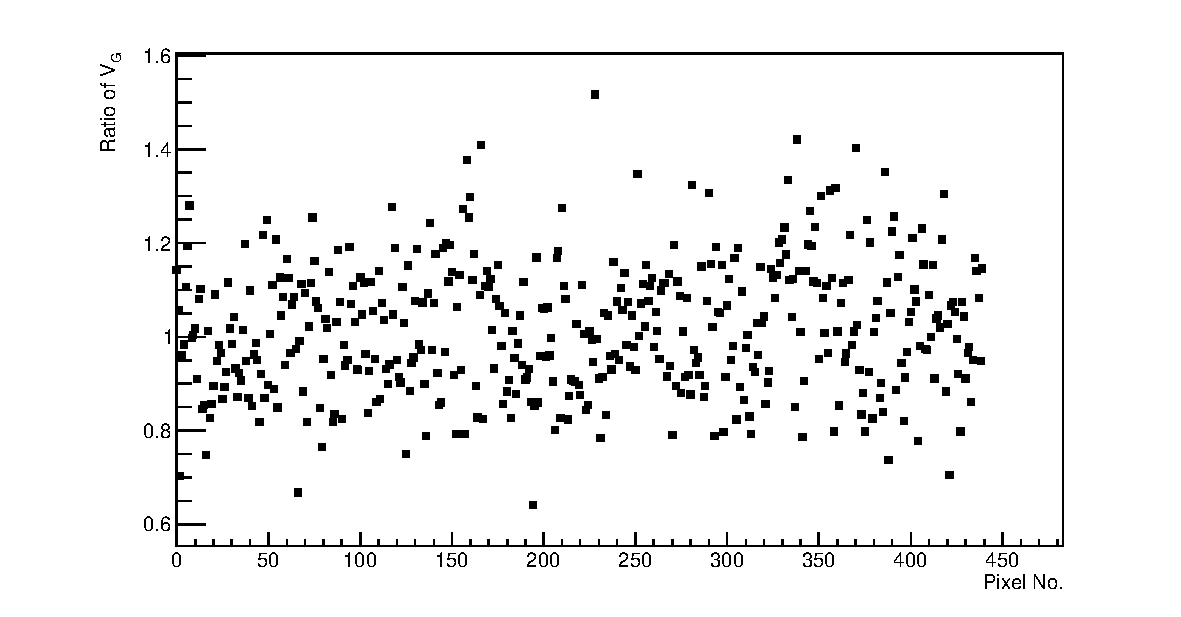
\includegraphics[width=\textwidth]{chapters/graphs/GainVarsMeas/LL_m04_2016-06-11/Set0and2/GainVars_Vs_Pixel_GainVariance_Average_Method2_Set0and2.pdf}
\caption{}
\end{figure}

\section{Attempts to measure Gain Variance directly in the Lab}